

\title{ROS2 for Robot Mapping and Navigation}
\author{
        Zoe Li \\
                Sunnyvale CA USA\\
}
\date{\today}

\documentclass[12pt]{article}

\usepackage{graphicx}
\graphicspath{{./graph/}}
\renewcommand{\thesection}{\Roman{section}}
\renewcommand{\thesubsection}{\thesection.\Roman{subsection}}


\begin{document}
\maketitle

\begin{abstract}
 This guide gives an overview of ROS2 status with an example of SLAM implementation. ROS2 is an upgrade after one decade since the introduction of ROS (Robotic Operating System) and is still under heavy development at this moment as June 2019. In this guide, we discuss and evaluate some of its new features by implementing SLAM in ROS2 in simulation and on a real robot. These new features are briefly introduced and some are tested in this implementation. A demo with source code is provided in the end of the paper.
\end{abstract}

\section{Introduction}
\subsection{Robot Operating System Background}
Robot Operating System (ROS) is a robotics middleware that was created by Willow Garage and Stanford University and now maintained by Open Source Robotics Foundation(OSRF).  As an open source framework for various robotics software development, ROS provides functions such as hardware abstraction, device control, message passing, package management and libraries for different functionalities. The modularity of ROS allows users to focus on application development rather than spending much effort to reinvent the wheel.

\subsection{ROS2 Design Background}
ROS was originally designed for PR2 use case. PR2 robot works as a standalone robot with excellent network connectivity, also PR2 applications are mostly research based, therefore the early design concept of ROS does not need to consider real-time problems.

Nowadays ROS has gained tremendous popularity in robotics community, and the use cases has grown beyond the scope of academia and scientific research. Many robotics applications such as  industrial robots, outdoor robots(for example driverless cars), unmanned aerial vehicles(UVA) have become more and more complicated, as a result, those applications have higher demand on the robust real-time performance of the robot operating system. Although ROS1 is still a very popular development tool in the field of robotics, the limitations of the original design have become a driving force of the new ROS2 design. 

With the growing demand of cross operating system platform and real-time functionality from the ROS community, ROS2 development was first announced at ROSCon 2014, and the first alpha version was launched in August 2015. On December 8, 2017, the highly anticipated ROS 2.0 finally released its first official version, Ardent Apalone. As of 2019, the newest version ROS 2 Dashing Diademata was released on May 30.

Compare to ROS1, ROS2 has the following support for robotics applications: 
\begin{itemize}
  \item \textbf{Cross-system platform support}: ROS2 support for Linux, Windows and macOS as well as the real-time operating system(RTOS).
  \item \textbf{Multi-robot system support}: Improved communication system allows robust network performance for multi-robot system 
  \item \textbf{Real-time control}: support to improve the timeliness of a robot control application and overall robot performance
  \item \textbf{Non-ideal networks}:
  \item \textbf{Production environments}:
  \item \textbf{Small embedded platforms}:
\end{itemize}
 


\subsection{ROS2 Communication}

\begin{figure}
  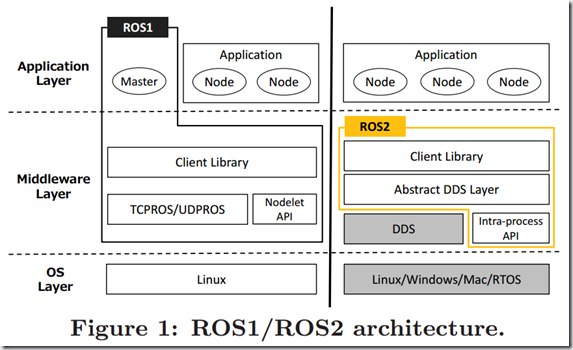
\includegraphics[width=\linewidth]{ros1_ros2_architecture.png}
  \caption{ROS1/ROS2 Architecture}
  \label{fig:boat1}
\end{figure}

ROS1 uses TCP (Transmission Control Protocol) as its communication protocol. TCP is a connection oriented network, this means that TCP tracks all data sent, requiring acknowledgment for each octet (generally), therefore,  ROS1 has a centralized network configuration which requires a running ROS master to take care of naming and registration services. With the help of the master, ROS nodes could find each other on the network and communicate in a peer-to-peer fashion. In ROS1 setting, all nodes will depend on the central ROS master. When the network becomes lossy and unstable(especially if nodes are distributed on several computers), the communication will not be reliable for real-time applications or multi-robot systems.

ROS2 uses Data Distribution Service (DDS) as the communication middleware. UDP is a Data-Centric-Publish-Subscribe(DCPS) model, and this model will create global data space for individual applications to exchange information. DDS will identify a data object by its topic name and then subscribe to this topic, therefore, DDS does not have a central distributor for all information. The DDS publish-subscribe model avoids complex network programming for distributed applications.  ROS2 provides an abstraction layer of DDS, so users do not need to pay attention to the underlying DDS structure. The ROS2 Middleware Interface(RMW) allows users to choose different Quality of Service(QoS). The real-time publish-subscribe (RTPS) protocol allows ROS2 nodes to automatically find each other on the network, thus there is no need for a ROS2 master. This is an important point in terms of fault tolerance.


% \paragraph{Outline}
% The remainder of this article is organized as follows.
% Section~\ref{previous work} gives account of previous work.
% Our new and exciting results are described in Section~\ref{results}.
% Finally, Section~\ref{conclusions} gives the conclusions.

\section{Related Work}\label{related Work}
A much longer \LaTeXe{} example was written by Gil~\cite{Gil:02}.

\section{Method}\label{method}
\section{Results}\label{results}
In this section we describe the results.

\section{Conclusions}\label{conclusions}
We worked hard, and achieved very little.

\section{Reference}\label{reference}
\bibliographystyle{abbrv}
\bibliography{main}

\end{document}